\subsection{Nah-seitige perspektivische Projektion}
\label{sec:nearsideperspective}
Die Nah-seitige Perspektive zeigt die Erde aus der Sicht eines Satelliten. Also ist es im Prinzip das selbe
wie die geostationäre Projektion. Allerdings muss der Satellit nicht über dem Äquator sein.\\

\begin{figure}[hbtp]
\centering
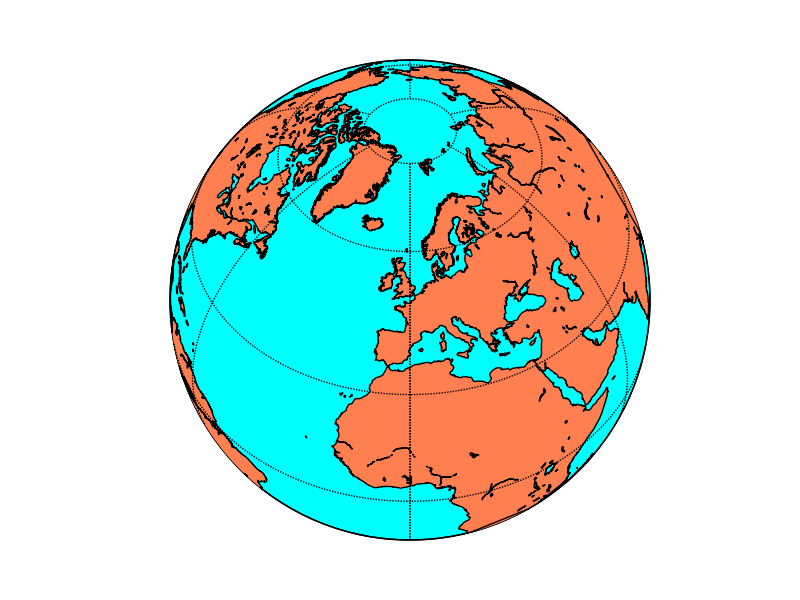
\includegraphics[scale=0.5,origin=c]{/Users/student/seminar/Kartendarstellungen/seminar/nearsid} \caption{Nah-seitige perspektivische Projektion}
\end{figure}
\newpage 